% DO NOT COMPILE THIS FILE DIRECTLY!
% This is included by the other .tex files.

\begin{frame}[t,plain]
\titlepage
\end{frame}

\begin{frame}
	\frametitle{Agenda}
	\begin{itemize}
        \item The pivotal role of interoperability in threat intelligence sharing
		\item MISP Standard format: designed for interoperability
		\item Interoperability mechanisms
        \item Data feeding mechanisms
	\end{itemize}
\end{frame}

\section{Interoperability in threat \\ intelligence sharing}

\begin{frame}
    \frametitle{The pivotal role of interoperability in threat intelligence sharing}
    \begin{itemize}
        \item Ensuring a \textbf{seamless flow of information} between tools
        \begin{itemize}
            \item Efficiency in information sharing
            \item Enables faster dissemination of threat intelligence
        \end{itemize}
        \item Enabling the scalability of the CTI pipeline with the integration of more tools
        \begin{itemize}
            \item Flexibility in the choice of tools
            \item More comprehensive view of threats
        \end{itemize}
        \item Fostering \textbf{collaboration}
        \begin{itemize}
            \item Encouraging the sharing of information
            \item Can lead to faster response to threats
        \end{itemize}
    \end{itemize}
\end{frame}

\begin{frame}
    \frametitle{Important features improving interoperability}
    \begin{itemize}
        \item \textbf{Standardisation is key}
        \begin{itemize}
            \item Relying on \textbf{standard formats} is mandatory
            \item \textbf{Wide adoption} of these formats is highly encouraged
            \item \textbf{Conversion mechanisms} between formats are essential
        \end{itemize}
        \item Taking advantages of \textbf{automation tools}
        \begin{itemize}
            \item \textbf{Efficiency in detection and response} is highly dependent on automation
            \item \textbf{Automated conversion} between formats included in your CTI pipeline is crucial
            \item Providing automation mechanisms to all users is a vector for \textbf{more collaboration}
        \end{itemize}
    \end{itemize}
\end{frame}

\section{A generic Data Format designed for interoperability}

\begin{frame}
    \frametitle{MISP standard format}
    \begin{itemize}
        \item \textbf{JSON} format
        \item Designed for \textbf{flexibility} and \textbf{extensibility}
        \item []
        \item A combination of meta-models with \textbf{generic field names} to describe data structures
        \begin{itemize}
            \item Flexible to allow the description of any kind of information in a structured manner
            \item Adaptable to easily extend the format to new use-cases
        \end{itemize}
        \item []
        \item Ensuring \textbf{long term interoperability} with existing MISP software and other Threat Intelligence Platforms and tools
    \end{itemize}
\end{frame}

\begin{frame}
    \frametitle{MISP standard format}
    \begin{itemize}
        \item Events as simple containers for embedded information
        \begin{itemize}
            \item Can be an incident, a security analysis, a threat intelligence report, or anything else
            \item No semantic meaning attached to the event itself
            \item Meaning of an Event only \textbf{depends on the embedded information}
        \end{itemize}
        \item []
        \item Attributes as the granular pieces of information to describe IoCs
        \begin{itemize}
            \item Made up of a \textbf{category} - \textbf{type} - \textbf{value} triplet
            \item Category and type give meaning to the value
            \item Difference between IoCs and observed data relies on a flag
        \end{itemize}
    \end{itemize}
\end{frame}

\begin{frame}
    \frametitle{MISP object templates}
    \begin{itemize}
        \item \textbf{Simple containers} grouping MISP Attributes to describe more complex data points
        \begin{itemize}
            \item JSON format with generic meta information, such as the \texttt{name} and \texttt{meta-category}
            \item The meaning of each Attribute within the object is defined by the \texttt{object relation}
        \end{itemize}
        \item A generic templating system
        \begin{itemize}
            \item Commonly used templates are provided by default
            \item Easily \textbf{extensible} to new use-cases
            \item Users can create \textbf{their own templates}
        \end{itemize}
        \item Include a vocabulary to describe the various \textbf{inter object and object to attribute relationships}
    \end{itemize}
\end{frame}

\begin{frame}
    \frametitle{MISP Taxonomies and Galaxies}
    \begin{itemize}
        \item Taxonomies are ensuring the \textbf{consistency} of the tags used in MISP
        \begin{itemize}
            \item Providing a \textbf{global classification} of data
            \item \textbf{Reused by other tools} interacting with MISP
        \end{itemize}
        \item []
        \item MISP Galaxies provide a way to attach \textbf{more complex structures} to MISP data
        \begin{itemize}
            \item They basically are tags with meta information
            \item Describing known threat actors, malware, techniques or other collections of \textbf{contextual information}
            \item MISP uses the tag name derived from the Galaxy Cluster
            \item Support for \textbf{custom} Galaxy Clusters
        \end{itemize}
    \end{itemize}
\end{frame}

\section{The support of focused specific formats}

\begin{frame}
    \frametitle{Supporting several patterning languages \& \\ signature formats}
    \begin{itemize}
        \item Provide information on how data has been detected/extracted in addition to the actual data
        \item Including:
        \begin{itemize}
            \item Yara \& Sigma signatures
            \item Snort / Suricata \& Zeek (previously Bro) rules
            \item STIX patterns
        \end{itemize}
        \item []
        \item Each of these formats is a \textbf{specific attribute type} in MISP
        \item Given rules, patterns and signatures can be extracted from MISP and \textbf{used to feed the respective tools}
    \end{itemize}
\end{frame}

\section{Several automation tools to \\ support interoperability}

\begin{frame}
    \frametitle{RESTfull APIs / PyMISP}
    \begin{itemize}
        \item Export \textbf{data collections} from MISP
        \begin{itemize}
            \item Enabled for several data structures - Events, Attributes, Galaxies, etc.
            \item Default format is \textbf{MISP standard - JSON}
            \item Supports a wide range of other formats, including \texttt{CSV}, \texttt{XML}, \texttt{Yara}, etc.
            \item \textbf{Advanced filtering capabilities}
            \item RESTfull API queries can be \textbf{automated} with \textit{curl} commands or \textit{Python} scripts using \textbf{PyMISP}
        \end{itemize}
        \item []
        \item Import data into MISP Events
        \begin{itemize}
            \item \textbf{Lossless} MISP JSON Events ingestion
            \item \textbf{PyMISP} can parse different formats too and convert data into MISP format
        \end{itemize}
    \end{itemize}
\end{frame}

\begin{frame}
    \frametitle{An advanced STIX conversion feature}
    \begin{itemize}
        \item Works as a \textbf{built-in module}
        \begin{itemize}
            \item Convert any data collection to STIX
            \item Import STIX files into MISP
        \end{itemize}
        \item Supporting all STIX versions
        \begin{itemize}
            \item STIX 1.x - XML
            \item STIX 2.x - JSON
        \end{itemize}
        \item Continuous development on STIX 2.x to \textbf{improve the conversion capacities} following evolutions on the STIX standards as well as the extensions of the MISP standard format
        \item Filling the mapping gaps over time to \textbf{improve interoperability} between MISP and other tools supporting STIX, such as TAXII, or STIX feeds producers
        \item Standalone conversion ability with the \textit{Python} library\footnote{\url{https://github.com/MISP/misp-stix}}
    \end{itemize}
\end{frame}

\begin{frame}
    \frametitle{MISP modules\footnote{\url{https://github.com/MISP/misp-modules}}}
    \begin{itemize}
        \item \textbf{Simple Python scripts} to automate the \textbf{import/export} of data
        \begin{itemize}
            \item Extending the range of supported formats
            \item Allows anyone to build their own module to either:
            \begin{itemize}
                \item Populate MISP Events with data from external sources/formats
                \item Extract and convert data from MISP Events
            \end{itemize}
        \end{itemize}
        \item Enrichment modules
        \begin{itemize}
            \item Use-case examples:
            \begin{itemize}
                \item \textbf{enrich} data with additional context
                \item \textbf{cross-reference} data with external sources
                \item \textbf{validate} data
            \end{itemize}
            \item Can be triggered automatically by \textbf{Workflows}
        \end{itemize}
    \end{itemize}
\end{frame}

\begin{frame}
    \frametitle{MISP Workflows}
    \begin{itemize}
        \item Needs that Workflows can address:
        \begin{itemize}
            \item Prevent default MISP behaviors
            \item Trigger specific actions to run callbacks
        \end{itemize}
    \end{itemize}
    \begin{center}
        \frame{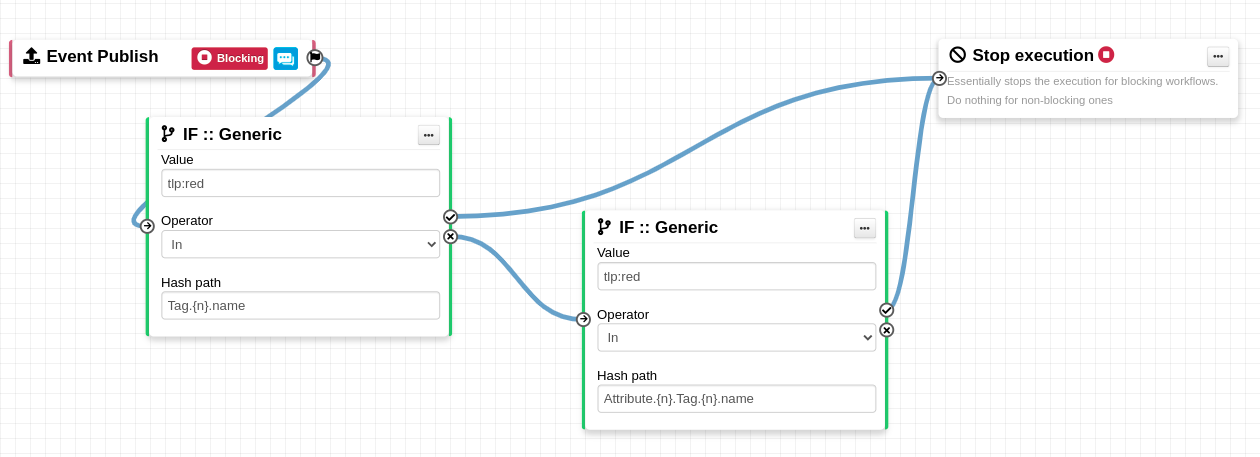
\includegraphics[width=1.0\linewidth]{../images/workflow.png}}
    \end{center}
\end{frame}

\begin{frame}
    \frametitle{PubSub channels}
    \begin{itemize}
        \item ZeroMQ channels
        \begin{itemize}
            \item N-to-N Asynchronous message-processing tasks
            \item Publisher(MISP) and consumer (scripts)
        \end{itemize}
        \item []
        \item \textbf{Streaming data as it is created in MISP}
        \item Advantage is the subscriber can \textbf{automatically use the published data}
        \item Be careful though with data being \textbf{republished}
        \item Also, there is \textbf{no access control} on the data that is streamed
    \end{itemize}
\end{frame}

\section{Data feeding mechanisms}

\begin{frame}
    \frametitle{Synchronisation between MISP instances}
    \begin{itemize}
        \item \textbf{Synchronisation is the default communication mechanism between MISP instances}
        \begin{itemize}
            \item Exchance of MISP standard format
            \item \textbf{Bidirectional} communication
            \item \textbf{Filtering} capabilities
        \end{itemize}
        \item Multiple data structures can be synchronised
        \begin{itemize}
            \item \textbf{Events are synchronised by default} with their \textbf{Attributes} \& \textbf{Objects}
            \item Synchronisation of Galaxy Clusters, Analyst Data \& Sightings can be enabled/disabled
        \end{itemize}
    \end{itemize}
\end {frame}

\begin{frame}
    \frametitle{Syncing / caching}
    \begin{itemize}
        \item \textbf{2-Step} process when Pulling Events
        \begin{itemize}
            \item Caching of the data
            \begin{itemize}
                \item Lookup of the Events in the remote instance
                \item Correlations with the Attributes in my instance
            \end{itemize}
            \item Fetching data
            \begin{itemize}
                \item Pulling the Events with their content on my instance
            \end{itemize}
        \end{itemize}
        \item Automated pushing mechanism
        \begin{itemize}
            \item \textbf{Published Events} and their content are pushed to the remote instance(s)
            \item Users can manually push Events
        \end{itemize}
    \end{itemize}
\end{frame}

\begin{frame}
    \frametitle{MISP Feeds\footnote{\url{https://www.misp-project.org/feeds/}}}
    \begin{itemize}
        \item MISP Feeds provide a way to:
        \begin{itemize}
            \item \textbf{Exchange information via any transport method} (HTTP, TLP, USB key, etc.)
            \item Preview events along with their attributes, objects
            \item Select and import events
            \item \textbf{Correlate attributes using caching}
        \end{itemize}
        \item []
        \item Feeds work without the need of MISP synchronisation
        \item \textbf{Feeds can be produced without the need of a MISP instance}
    \end{itemize}
\end{frame}

\begin{frame}
    \frametitle{References}
    \begin{itemize}
        \item References on the presented topics
        \begin{itemize}
            \item MISP Standards: \url{https://www.misp-standard.org/standards/}
            \item MISP Concepts Cheat sheet: \url{https://www.misp-project.org/misp-training/cheatsheet.pdf}
        \end{itemize}
        \item More details on MISP
        \begin{itemize}
            \item Contact: \url{info@circl.lu}
            \item \url{https://www.misp-project.org}
            \item \url{https://github.com/MISP}
        \end{itemize}
    \end{itemize}
\end{frame}
